\section{Способы процедурной генерации сцены}

\subsection*{Алгоритм квантового коллапса волновой функции}

Алгоритм квантового коллапса волновой функции (далее - QWFC или WFC) — это метод генерации контента, который используется для создания двумерных и трёхмерных структур, таких как уровни в видеоиграх, текстуры и другие элементы. Он был разработан Максимом Гуминым и основан на концепциях из квантовой механики, хотя и не имеет прямого отношения к физике~\cite{QWFC}.

\begin{wrapfigure}{r}{0.39\textwidth}
  
  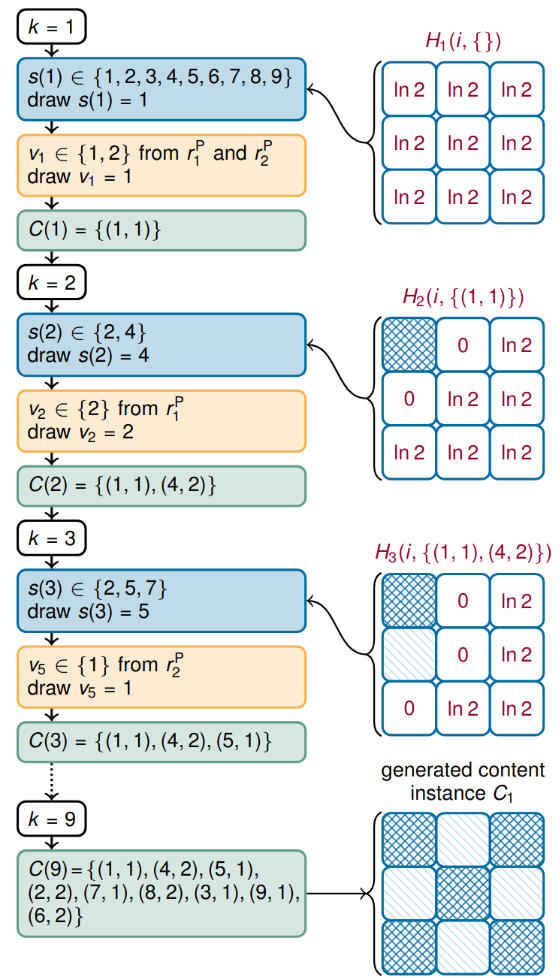
\includegraphics[width={.39\textwidth}]{generation_example.png}
  \caption{Пример работы алгоритма QWFC}
  \label{fig:qwfc_example}
\end{wrapfigure}

Алгоритм работает путём заполнения сетки, каждая ячейка которой может принять одно из определённых состояний. Для заполнения сетки требуется предопределённый набор правил и приоритетов, который описывает то, какие ячейки могут быть "соседями" других ячеек. Изначально все ячейки находятся в состоянии суперпозиции -- каждая может принять любое состояние (отсюда происходит слово "квантовый" в названии алгоритма). Затем, у случайной ячейки фиксируется одно из состояний (которое также выбирается случайно, но есть возможность задать приоритеты для тех или иных состояний). На основе этой зафиксированной ячейки, обновляется состояние остальной сетки, чтобы учесть появившиеся ограничения. Цикл повторяется, пока сетка не будет заполнена.

Этот алгоритм подходит для выполнения поставленной задачи (генерации загородного посёлка), так как он позволяет нам заполнить заданную плоскость в соответствии с ограничениями, а также предоставляет возможность влиять на результат посредством коэффициентов, которые можно задавать в пользовательском интерфейсе.

На рисунке~\ref{fig:qwfc_example} изображён пример работы алгоритма QWFC для создания изображения размера 3 на 3. В этом примере, возможны два типа ячеек --- закрашенная или незакрашенная. Правило соседства для каждого типа ячеек гласит: ячейка не может соседствовать с ячейкой того же типа. 

На рисунке число $k$ означает итерацию алгоритма. Множество $H$ --- множество пар чисел, описывающих номер ячейки и зафиксированный тип. $s$ --- множество ячеек с минимальным количеством состояний. $v$ --- возможное фиксируемое состояние ячейки. $C$ --- выходной список, описывающий состояние матрицы.